%%
%% This is file `esapub.tex',
%% generated with the docstrip utility.
%%
%% The original source files were:
%%
%% esapub.dtx  (with options: `manual')
%% ============================================
%% This is the manual describing the usage of
%%      esapub.cls
%% ============================================
%% Copyright 1999 Patrick W Daly
%% Max-Planck-Institut f\"ur Aeronomie
%% Max-Planck-Str. 2
%% D-37191 Katlenburg-Lindau
%% Germany
%% E-mail: daly@linmpi.mpg.de
%%
%% -------------------------------------------------
\ProvidesFile{esapub.tex}
          [2001/04/25 1.1 (PWD)]
\documentclass[a4paper,twocolumn]{esapub2005} % European paper
\pagestyle{empty}

% introduce this option for the ESA publications style
\bibliographystyle{alpha}

\usepackage{times}
\usepackage{natbib}
\usepackage{graphicx}

\title{An enhanced Soil Moisture product from ERS scatterometers}
\author{Christoph Reimer}
\author{Isabella Pfeil}
\author{Wolfgang Wagner}
\affil{TU Wien, Department of Geodesy and Geoinformation, Research Group Remote Sensing}

\newcommand{\btx}{\textsc{Bib}\TeX}
\newcommand{\filename}{esapub}

\begin{document}

\maketitle

\begin{abstract}
Talks presented at an ESA sponsored conference are published by the ESA
Publications Division by means of author-produced camera-ready copy. The
format is predetermined. This \LaTeX\ class allows authors to produce
this format with a straight-forward \LaTeX\ file. The only non-standard
features are the \verb!\keywords! command and the method for entering
author and affiliation names. \btx\ support is provided as a bibliography
style file for the publicly available package \texttt{natbib}.
\end{abstract}

\keywords{Soil Moisture;ERS;scatterometer}

\section{Introduction}
Active microwave remote sensing has a long heritage in the European earth observation programme, initiated with the launch of the European Remote Sensing satellite ERS-1 in 1991.
ERS-1 was equipped with a sophisticated C-band scatterometer (ESCAT) providing insights into ocean and land surface dynamics of the Earth.
Because of the great success of the ERS-1 mission, the follow-on mission ERS-2 was launched in 1995 carrying an identical constructed C-band scatterometer.
After 9 years of excellent performance, ERS-1 was decommissioned in the year 2000, followed by ERS-2 in 2011 after almost 16 years in space.
Global C-band scatterometer observations from ESCAT on-board of ERS-1 and ERS-2 comprise a unique data archive covering a period of about 20 years.
The first global soil moisture product from the scatterometer (ESCAT) on-board the ERS-1/2 missions was derived in the year 2002, by making use of the TU~Wien Soil Moisture algorithm~[1, 2].
The ERS missions, especially ERS-2, underwent a number of major mission events (Figure~\ref{figure:mission_events}) affecting the final Soil Moisture retrievals~[3].
In the framework of the ESA funded project SCIRoCCo, this data archive was reconsidered with the objective to create the most complete and consistent ESCAT soil moisture dataset, taking full advantage of state of the art scatterometer processing facilities.
 

In the framework of the ESA funded project SCIRoCCo (Scatterometer Instrument Competence Centre), this data archive was reconsidered with the objective to generate the most complete and consistent ESCAT dataset.
TU Wien is one of the project consortium members regarded as the reference laboratory for soil moisture (SM) retrieval from scatterometers.
Accordingly, TU Wien undertake the generation of an up-to-date ESCAT SM dataset based on re-processed Level 1 backscatter data.
In this study the major project achievements with respect to the production of the most complete ESCAT SM data archive are presented.
First, the high radiometric quality of the re-processed Level 1 backscatter data is demonstrated with reference to well defined calibration targets.
Furthermore, enhancements of the TU Wien soil moisture algorithm are discussed covering an improved SM error characterisation and improvements in the model parameter estimation.
Finally, results of a comprehensive validation of the obtained SM product in comparison to in-situ measurements and soil moisture estimates from land surface models are presented.

\begin{figure}
  \centering
  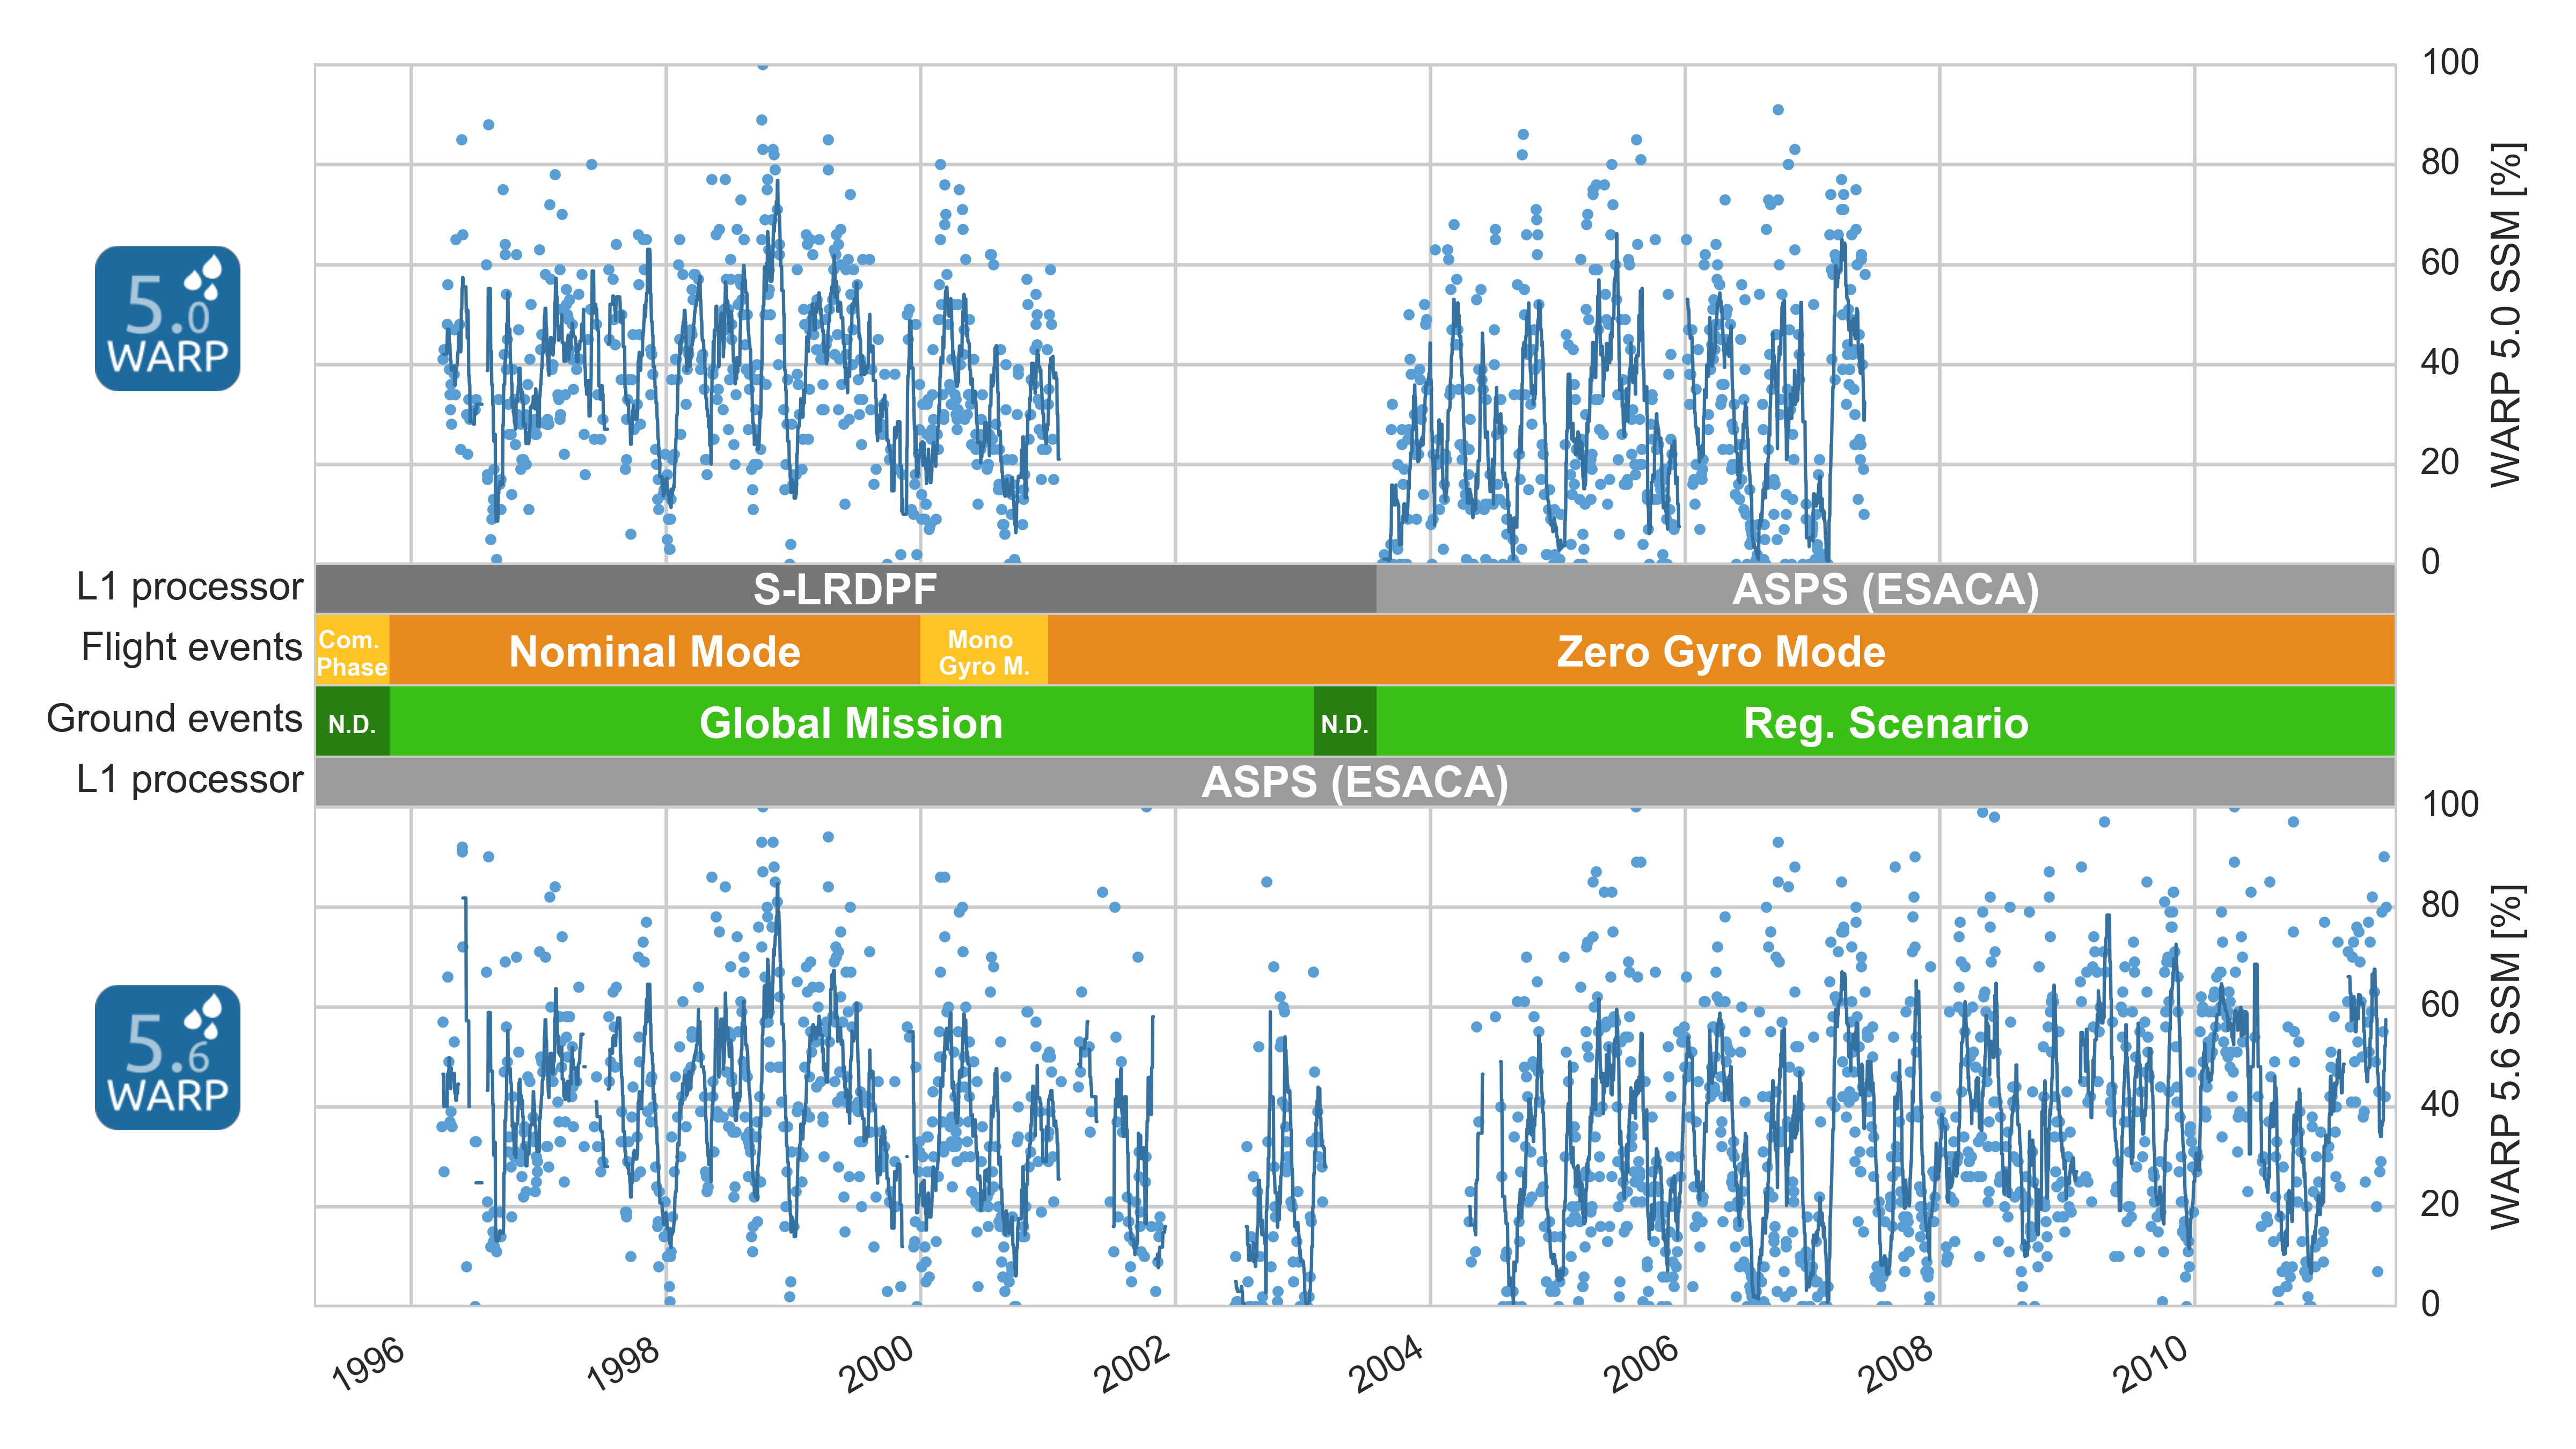
\includegraphics[width=1.\linewidth]{../poster/figures/ERS_mission_overview.png}
  \caption{Major mission events of ERS-2 and their effect on the final soil moisture retrievals from ESCAT.\@ Two major mission events should be noted, the loss of the 5 gyroscopes leading to the so called Zero Gyro Mode, and the on-board tape recorder failure resulting in the Regional Mission Scenario.\label{figure:mission_events}}
\end{figure}

\section{The WAter Retrieval Package (WARP)}
The TU-Wien soil moisture algorithm is a physically motivated change detection approach implemented in a software called the WAter Retrieval Package (WARP).
Since the first release of global soil moisture observations from ESCAT in 2002, algorithmic updates and improvements have been implemented into WARP.
In view of the SCIRoCCo project, latest algorithmic changes, previously specially tailored to ASCAT, have been adopted to extent the soil moisture retrieval capabilities also to ESCAT.
As a consequence, WARP was implemented from scratch in Python taking advantage of this community drive programming language and external packages.

The first step in the WARP processing chain has the objective to create backscatter time-series from the Level 1b ESCAT data in swath-geometry.
This is done by spatial interpolation (re-sampling) of the radar backscatter to a discrete global earth grid (DGG), which is a computation intensive task.
With respect to that, the spatial re-sampling strategy was completely redesigned with a strong focus on parallel processing capabilities in addition to updates in data quality and orbit propagation checks. 

In order to guarantee the consistency and stability of the Level 1 scatterometer observations, the normalized radar cross section, a sensor intra-calibration method is introduced [ref Master thesis].
The objective of intra-calibration is to detect and remove senor related biases of a specific or among different instrument antennas by making use of natural calibration targets such as the Amazon Rainforest.

The land surface state can change over the year mostly related to changes in temperature from freezing to thawing conditions or perhaps standing water on the surface.
To account for such land surface state changes affecting the backscatter and consequently the final soil moisture retrieval, a freeze/thaw classification step is introduced based on external temperature data from ERA-interim [ref to ERA-interim].
This classification was initially develop and tested for ASCAT and was updated and transferred recently to ESCAT.

Scatterometer Level 1 backscatter observations have to be normalised according to their observation geometry to make them comparable over time. Furthermore, the exploitation of a change detection algorithm for soil moisture retrieval requires knowledge about the driest and wettest observed backscatter. These references are assume to represent the backscatter for completely unsaturated soil conditions (dry-reference) and saturated soil (wet-reference).
Because of the importance of a robust estimation of the dry- and wet-reference this processing step was improved by making use of a statistical outlier detection scheme incorporating backscatter error estimates.

In very dry regions it is impossible to derive a realistic estimate of the wet-reference, because of the lack strong rain events resulting in completely saturated soil conditions. Therefore, a wet-correction is applied by facilitating an external climate map to identify such very dry regions like desserts. 

\begin{figure}
  \centering
  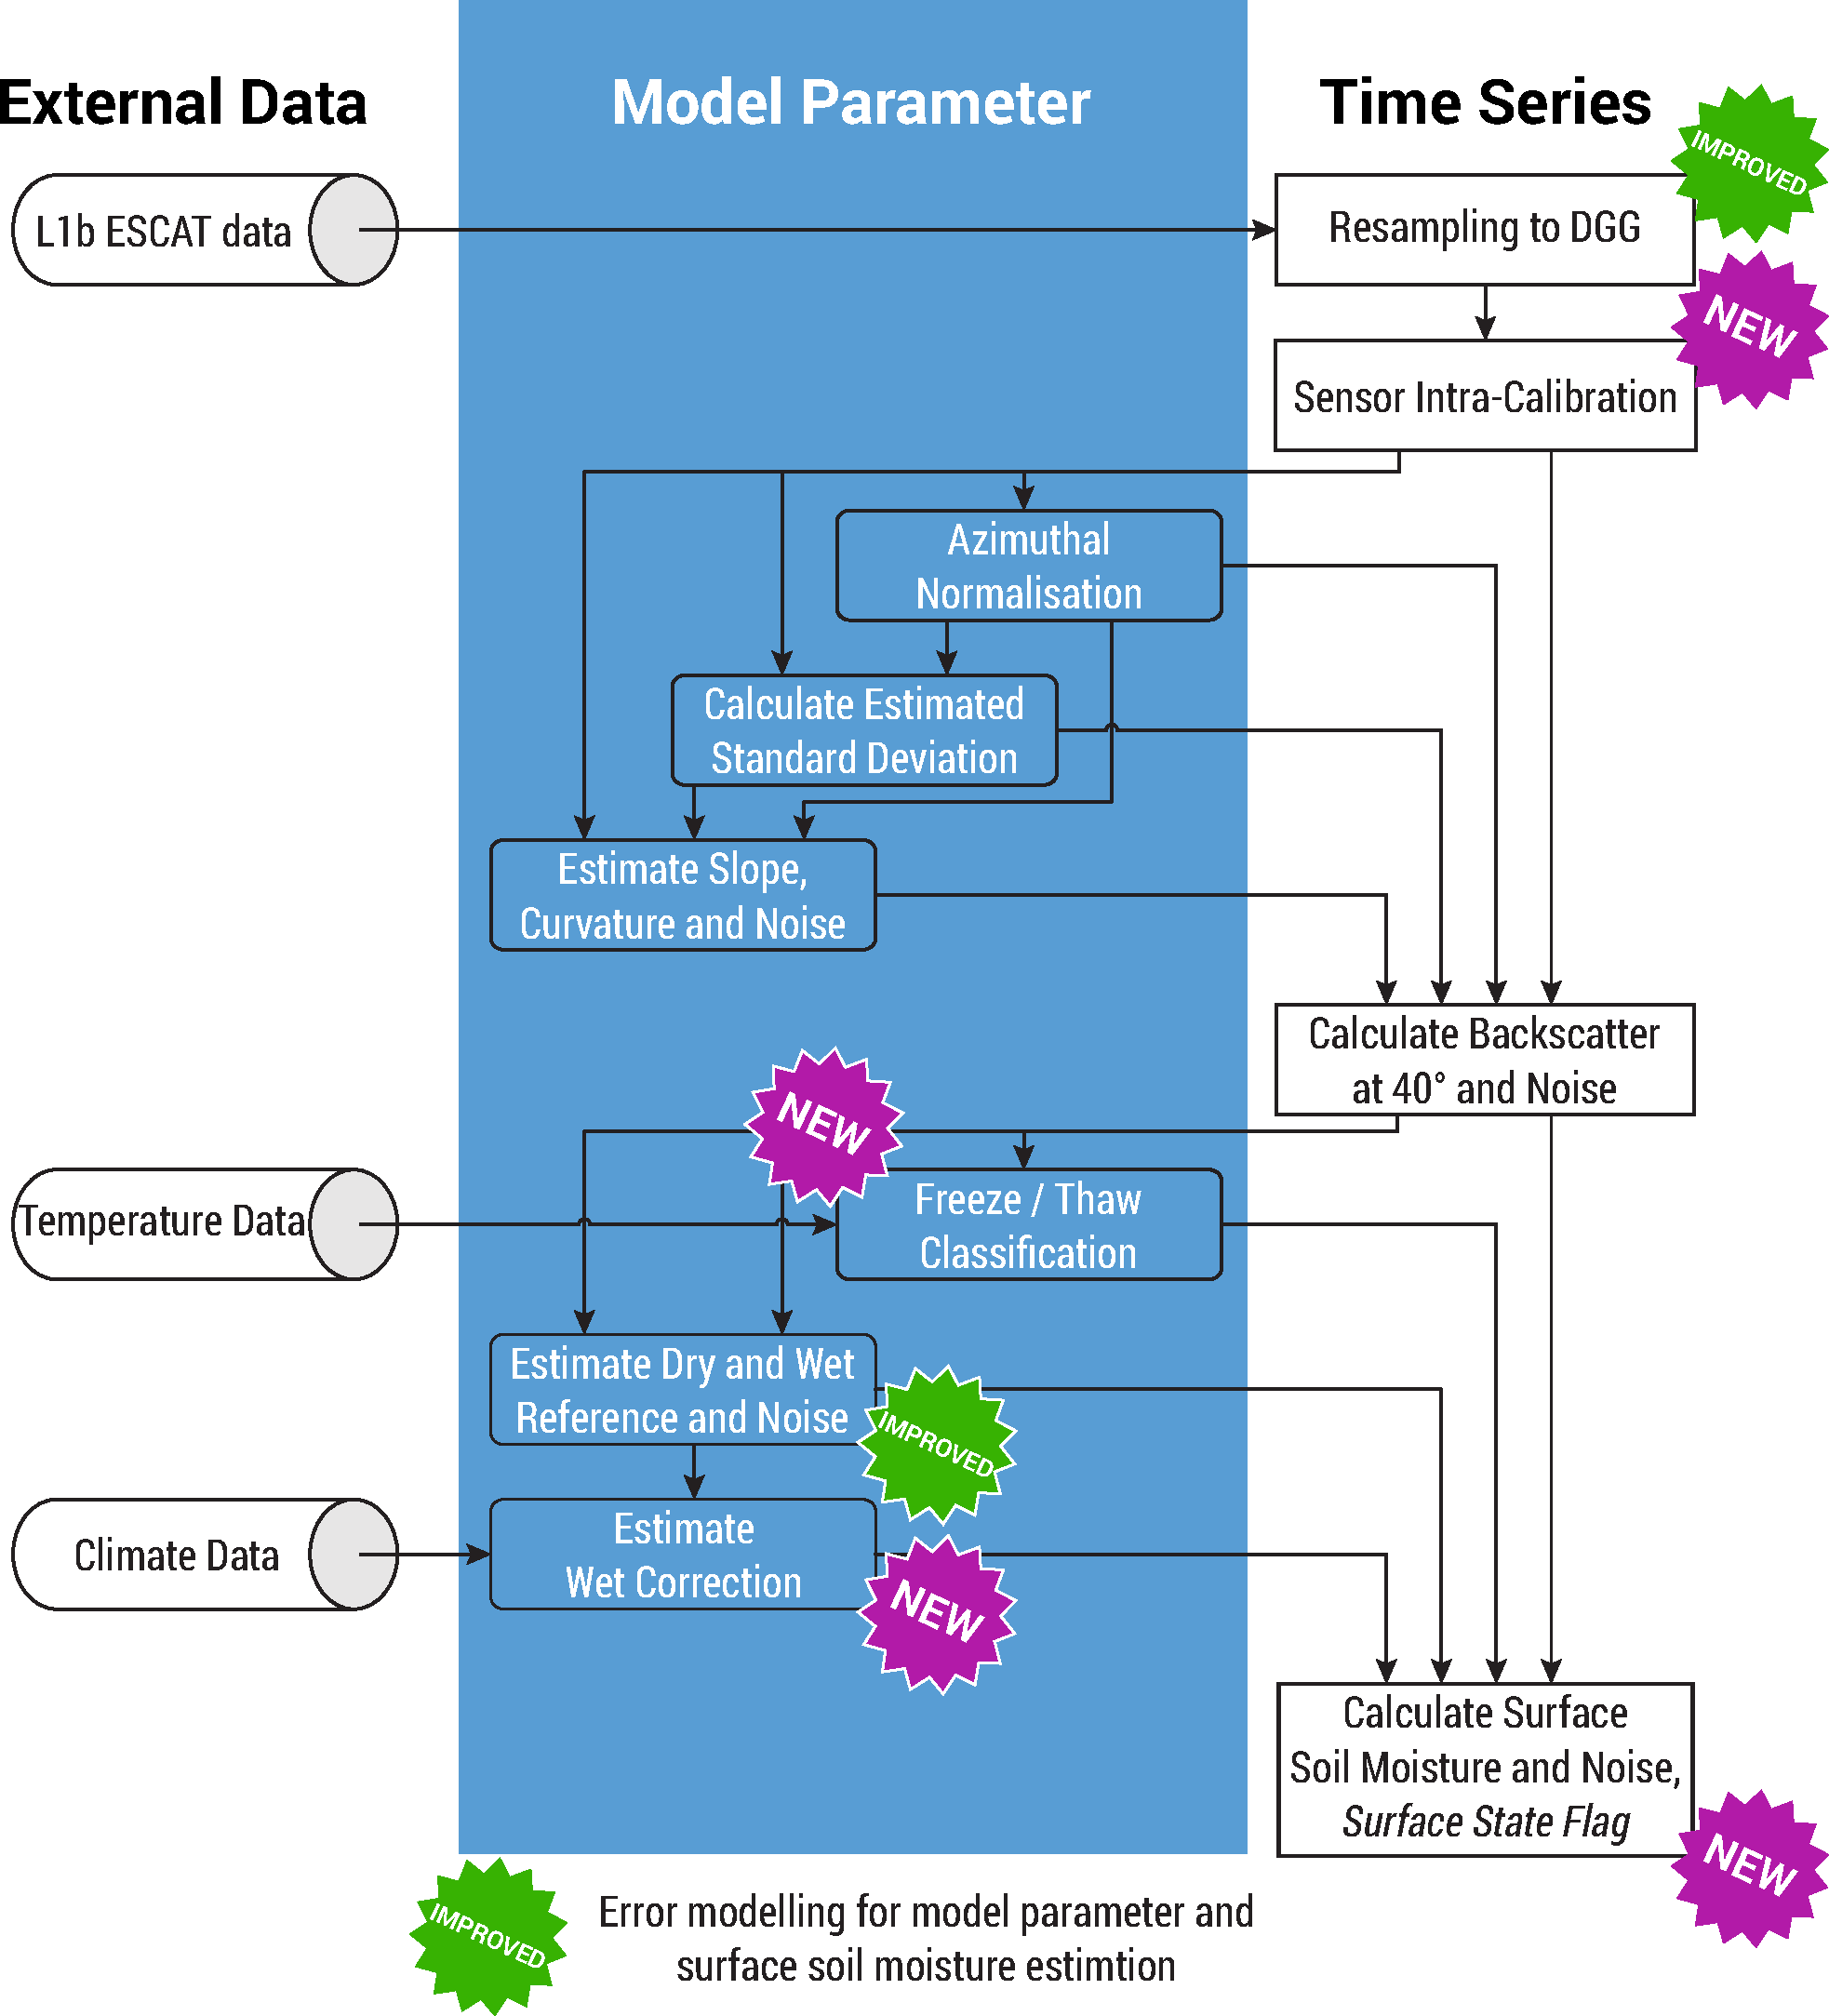
\includegraphics[width=1.\linewidth]{../poster/figures/WARP_processing_steps.pdf}
  \caption{Flow chart of the TU Wien soil moisture retrieval algorithm implemented in the WAter Retrieval Package (WARP). Indicated algorithmic changes and improvements are given with respect to the previous derived ESCAT soil moisture products based on WARP 5.0.\label{figure:flow_chart}}
\end{figure}  

\section{Product Overview}
Soil moisture products from ERS ESCAT have been re-processed resulting in a Swath-Grid and a Time-Series product to cover the wide range of applications (see Figure \ref{figure:escat_products}).
The Swath-Grid product is aimed for NWP centers in support to NWP re-analysis and climate monitoring activities (see Figure \ref{figure:spat_res}).
For research and climate change studies a Time-Series product is accessible located on a discrete global earth grid (see Figure \ref{figure:mission_events}).
Both soil moisture products are available at two different spatial resolutions with a sampling of 12.5 and 25 km (see Figure \ref{figure:spat_res}), and will be disseminated in NetCDF following the CF-conventions.\\

\begin{figure}
  \centering
  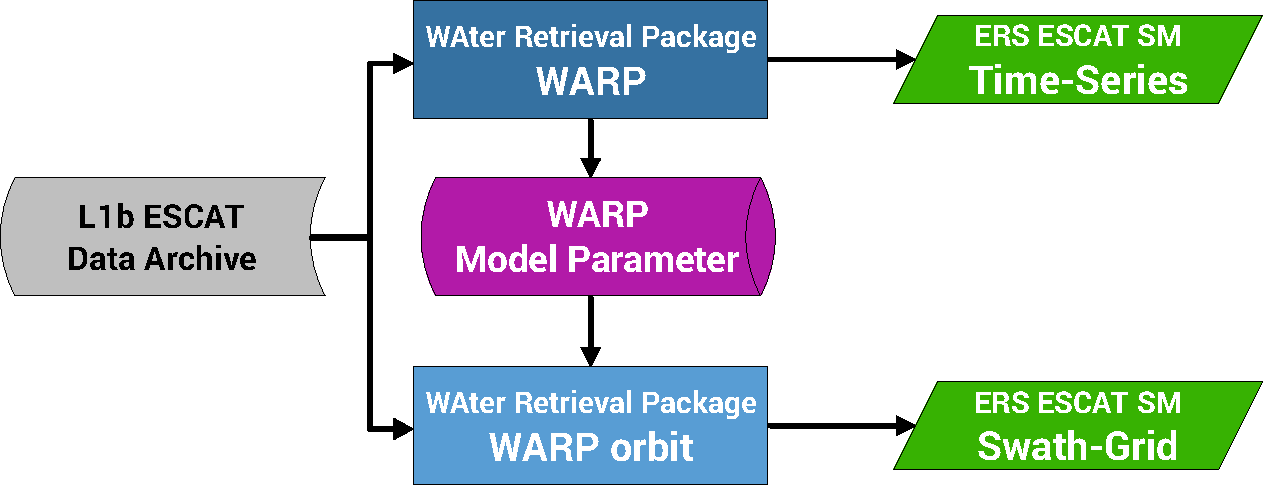
\includegraphics[width=1.\linewidth]{../poster/figures/WARP_WARPNRT.pdf}
  \caption{ERS ESCAT soil moisture product generation flow chart depicting the relationship between the Swath-Grid and Time-Series products.\label{figure:escat_products}}
\end{figure}

\begin{figure}
  \centering
  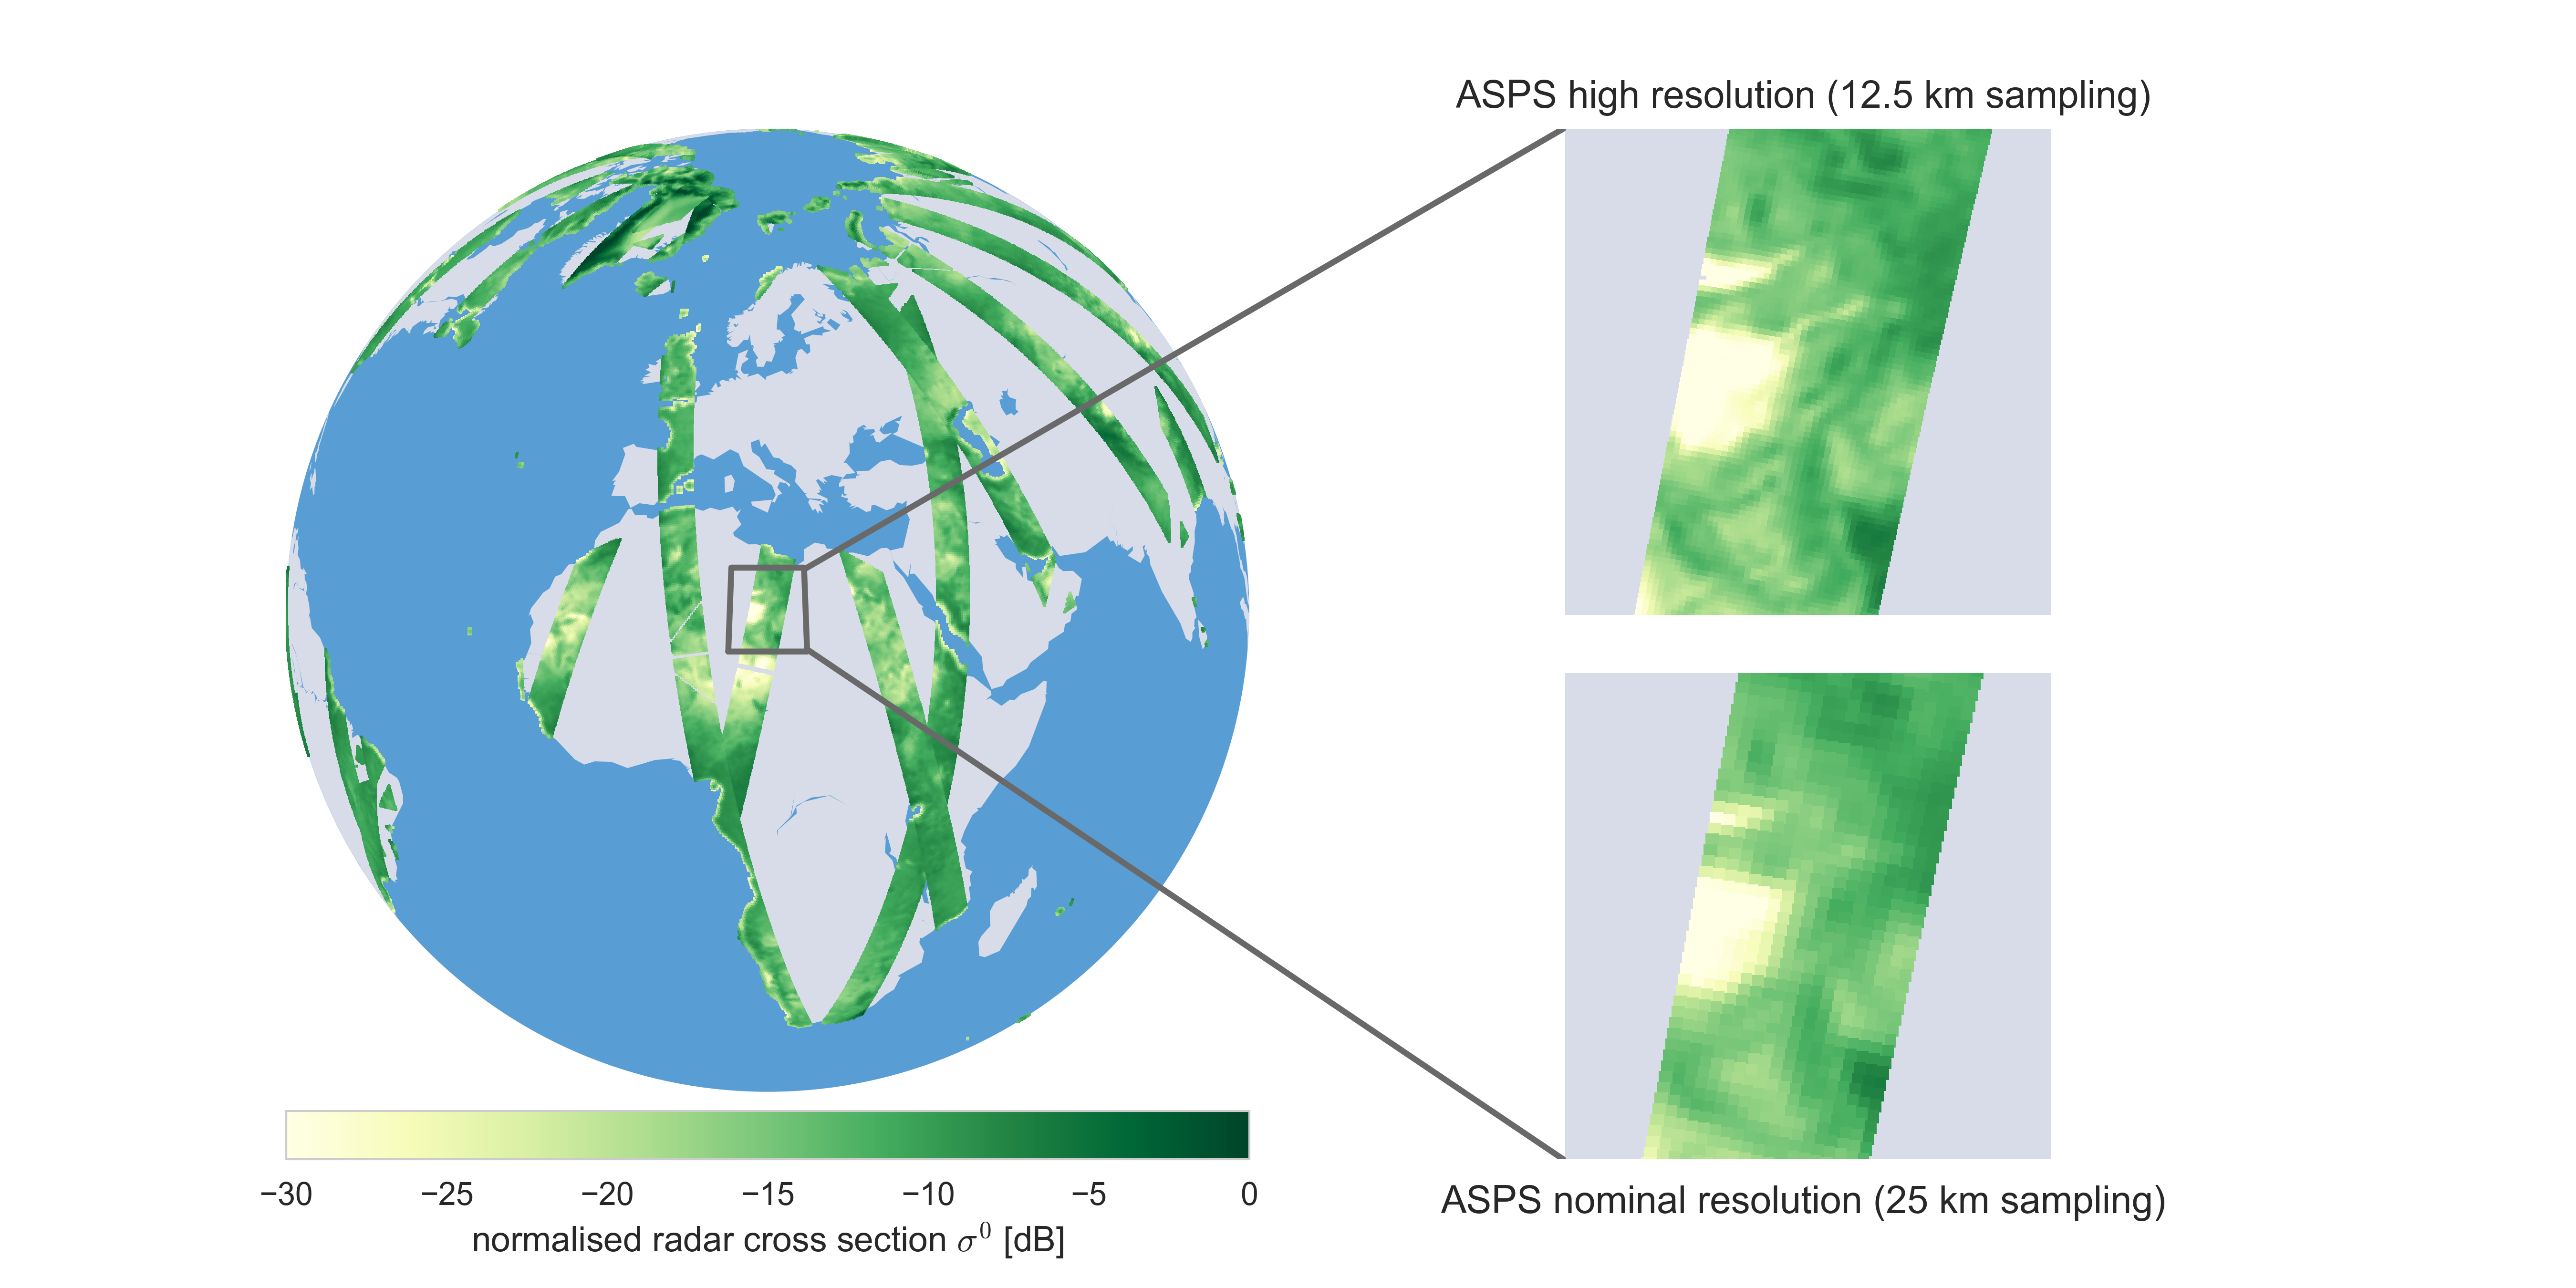
\includegraphics[width=0.9\linewidth]{../poster/figures/ASPS_resolutions.png}
  \caption{Illustration of the different spatial resolutions of the Level 1 input dataset used for soil moisture retrieval at TU~Wien.\label{figure:spat_res}}
\end{figure}


\section{Validation}

\begin{figure}
  \centering
  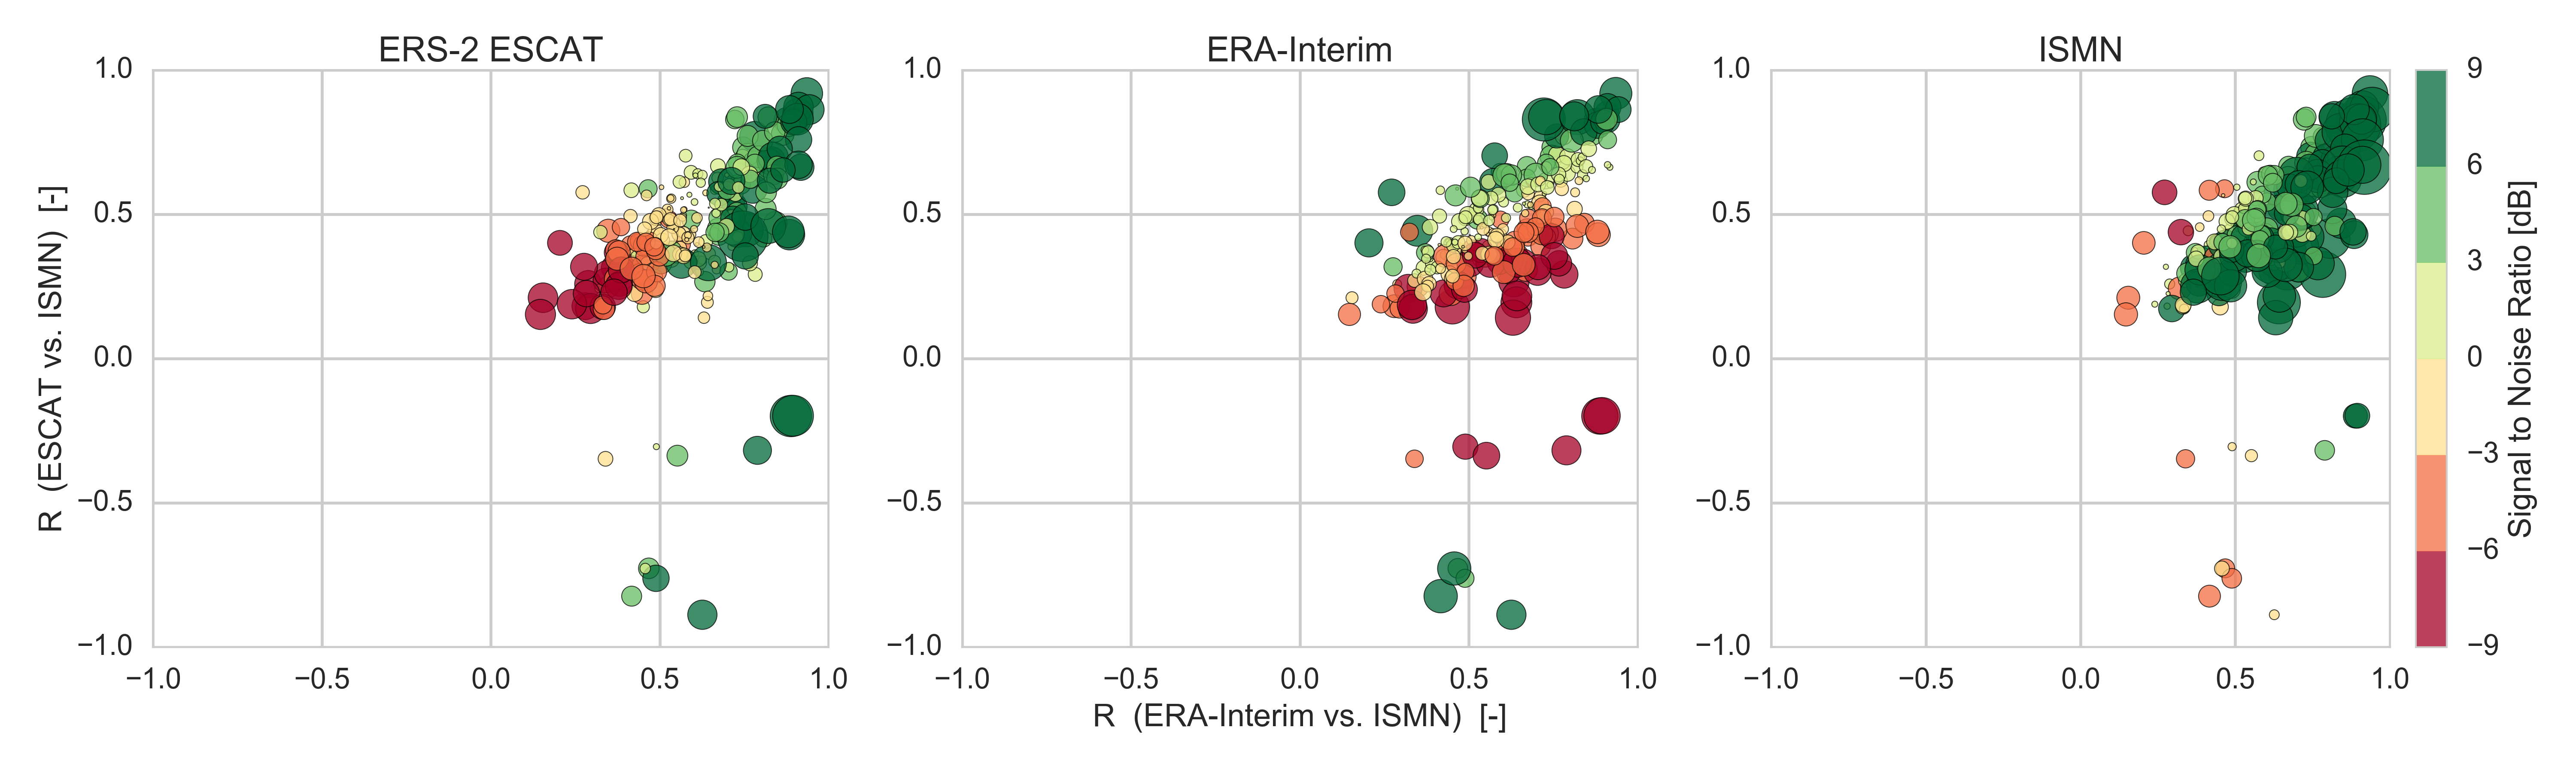
\includegraphics[width=1.\linewidth]{../poster/figures/TripleCol_SNR_R.png}
  \caption{ISMN validation results utilizing Triple Collocation technique to estimate the Signal to Noise Ratio (SNR) in addition to Pearson R coefficient. Results are only shown for statistical significant correlations~(p~$>$~0.05).\label{figure:ismn_val}}
\end{figure}

\begin{figure}
  \centering
  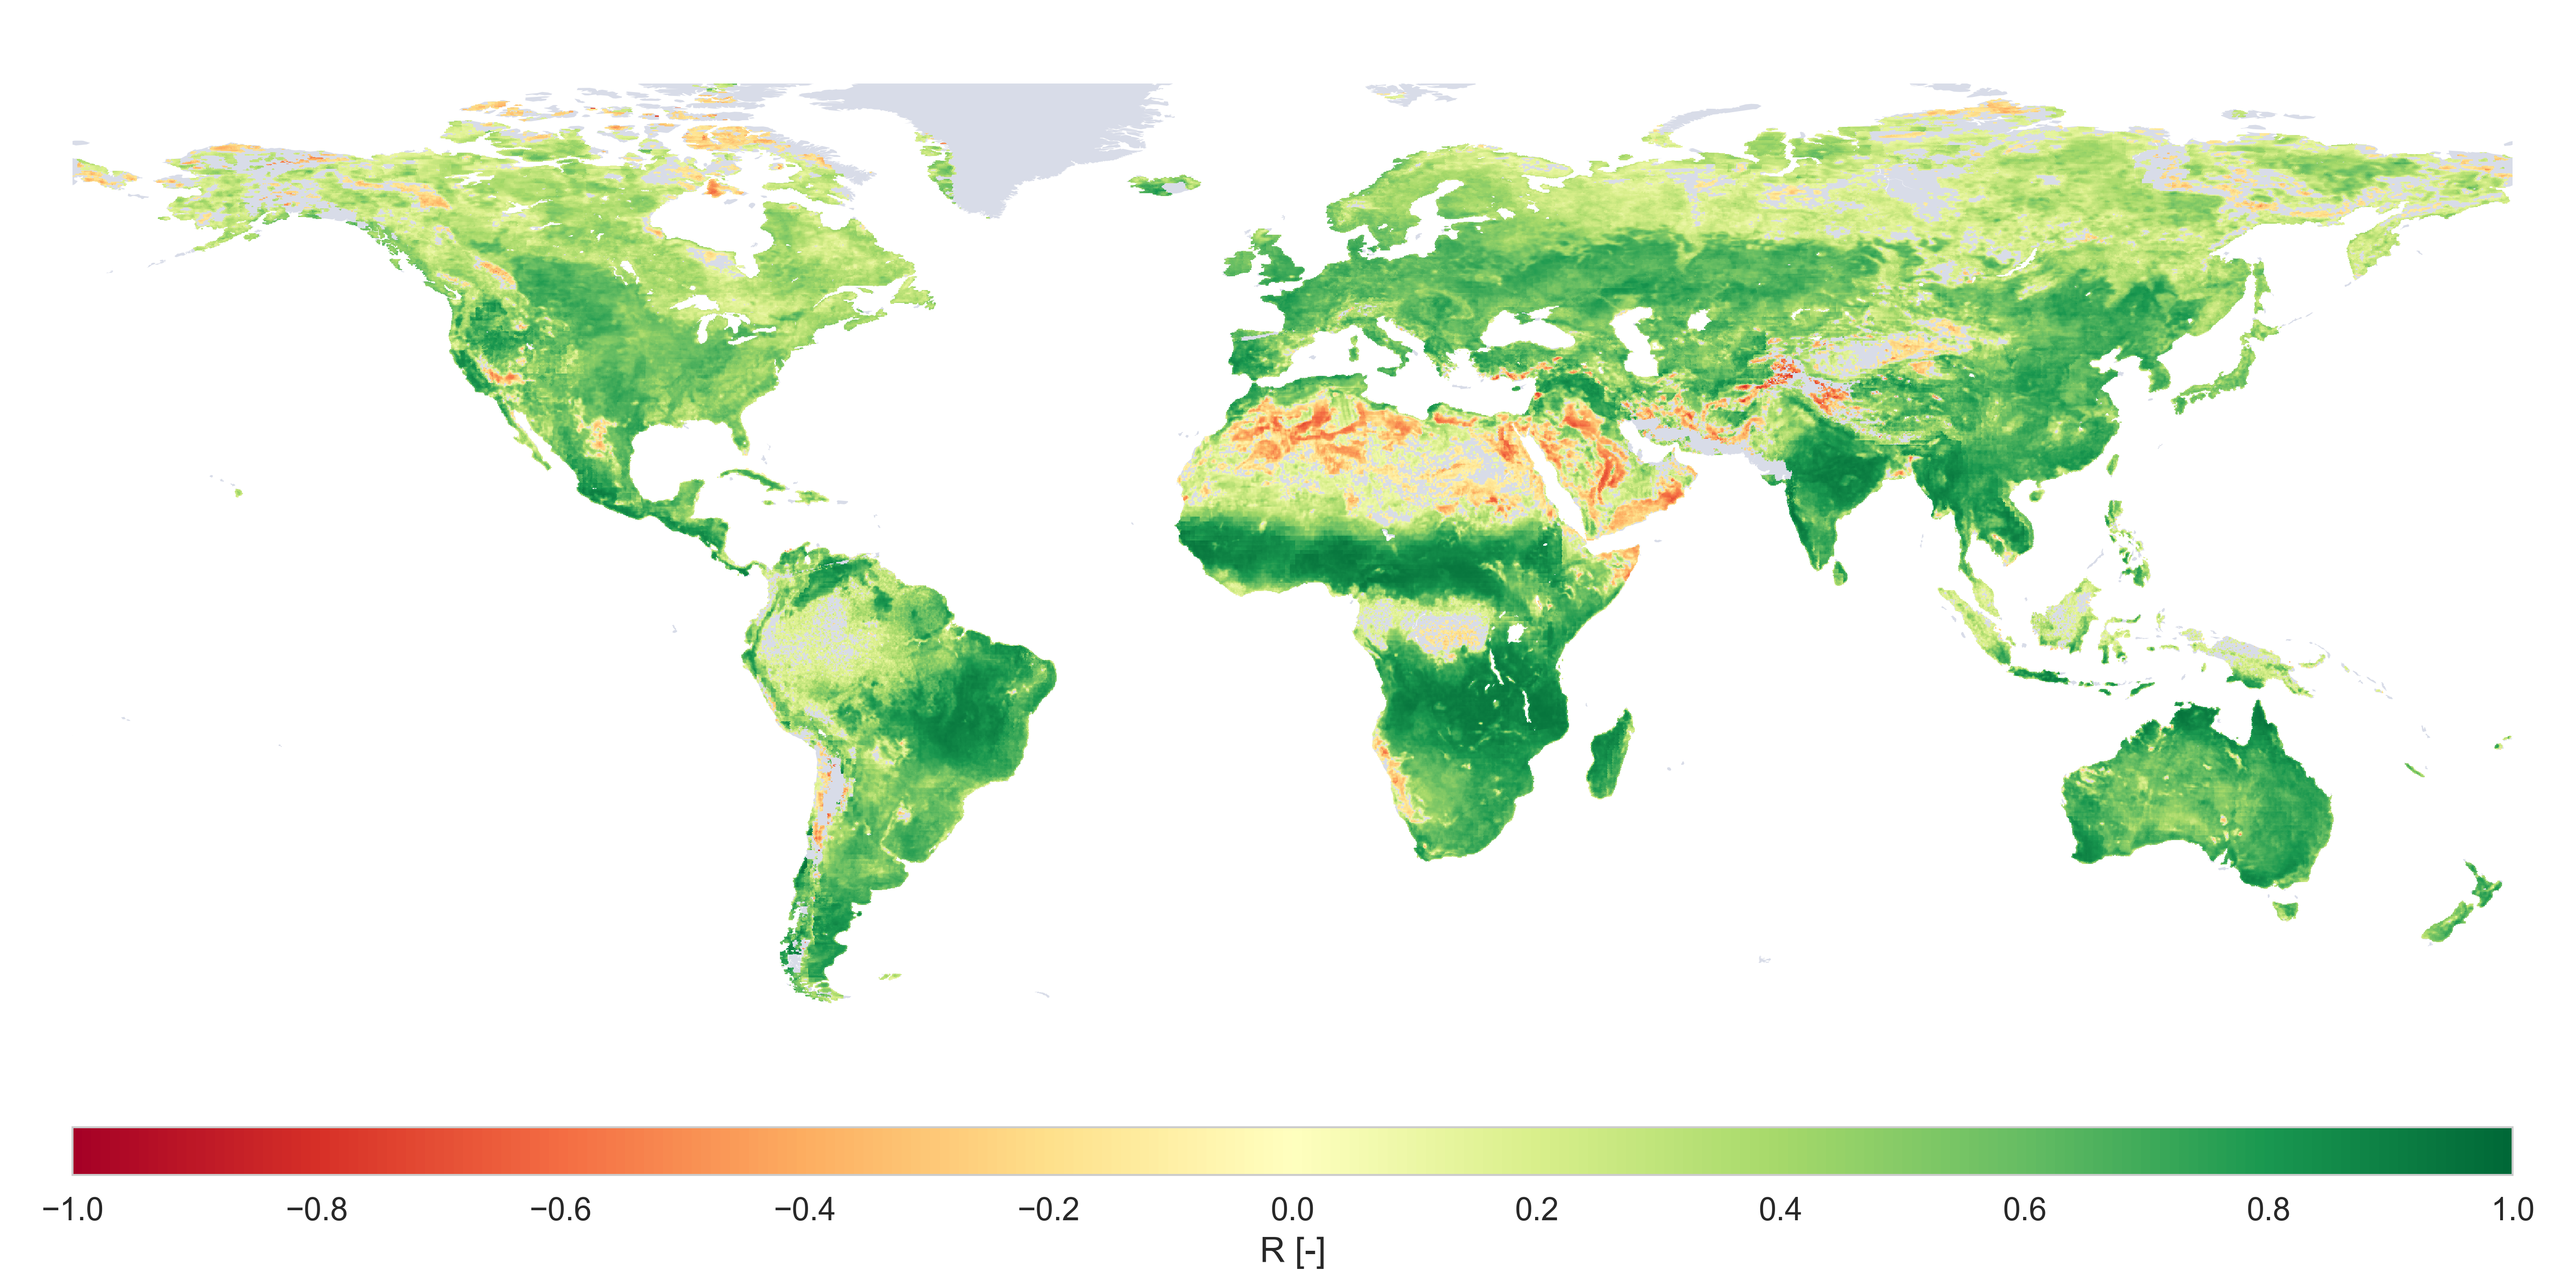
\includegraphics[width=1.\linewidth]{../poster/figures/WARP_SM_ERAINT_R_ALL_map.png}
  \caption{Pearson correlation coefficient R between the derived ESCAT soil moisture Time-Series and ERA-interim modeled soil moisture. Results are only shown for statistical significant correlations~(p~$>$~0.05).\label{figure:lsm_val}}
\end{figure} 

\section{Conclusions}

\section*{Acknowledgments}

\end{document}
%%
%% <<<<< End of generated file <<<<<<
%%
%% End of file `esapub.tex'.
